\subsubsection{Wstęp}
				\par Wykorzystując abstrakcyjny schemat komponentów systemu można utworzyć system komputerowy realizujący założoną funkcjonalność. Na podstawie schematu \ref{basic_comp} można przygotować listę programowych komponentów systemu komputerowego. Z powyższego schematu wynika wprost, że system komputerowy musi składać się z: systemu baz danych, systemu plików, centrali telefonicznej, systemu wiadomości e-mail, systemu zarządzania i sklepu internetowego.
				\par Niezbędne jest dodanie do listy składników elementów o znaczeniu technicznym. Będą nimi: system DNS (Domain Resolve System) z ang. system nazw domenowych, odpowiedzialny za tłumaczenie adresów domen na adresy IP. Jest to wymóg rfc1035, aby móc przechowywać domenę, oraz sieciowy system plików, który umożliwi przechowywanie wszystkich danych i współdzielenie ich pomiędzy składnikami systemu.
				
				\par Na podstawie dwóch poprzednich paragrafów można sprecyzować listę składników systemu komputerowego w następujący sposób:
				\begin{itemize}
					\item System DNS
					\item System wiadomości e-mail
					\item Bazy danych
					\item Centrala telefoniczna
					\item Współdzielony system plików
					\item Sklep internetowy
					\item System zarządzania
				\end{itemize}
				
				\begin{figure}[H]
					\centering
					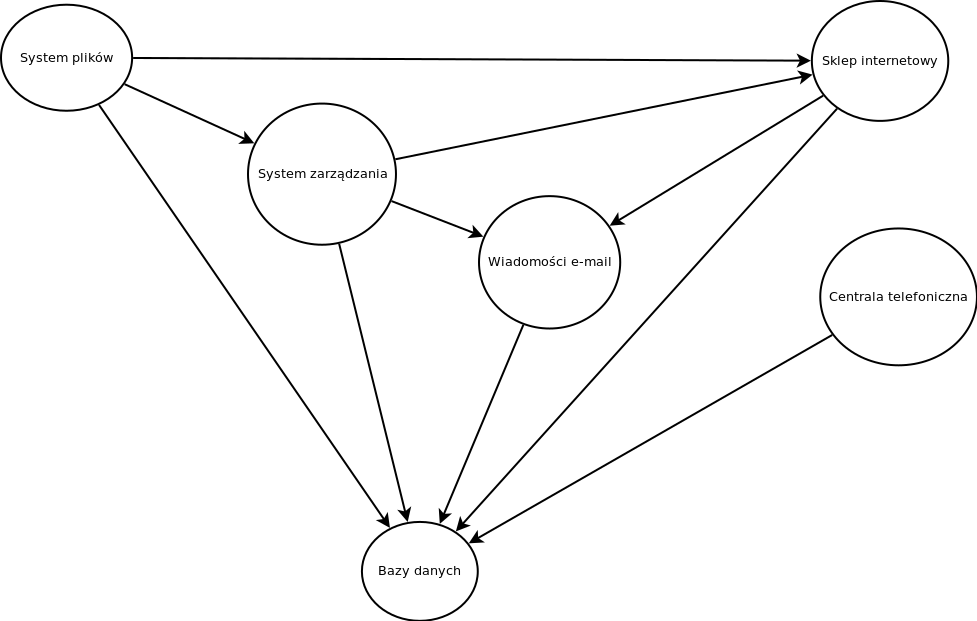
\includegraphics[width=\textwidth]{extended_comp}
					\caption{Schemat składników systemu komputerowego}
					\label{extended_comp}
				\end{figure}
			
			\subsubsection{Opis}
				\par Wymienione uprzednio składniki systemu komputerowego, którymi są: system DNS, system wiadomości e-mail, bazy danych, centrala telefoniczna, współdzielony system plików, sklep internetowy oraz system zarządzania umożliwiają komunikację między między pracownikami i klientami sklepu. Dzięki następującym funkcjonalnością:
				
				\begin{description}
						\item[System DNS] - system odpowiedzialny za przechowywanie domen sklepu internetowego, jego zadaniem jest kierowanie klientów do odpowiednich serwerów poprzez tłumaczenie zrozumiałych dla człowieka nazw na adresy występujące w sieciach komputerowych. Przykładem może być nazwa domenowa \textit{sklep-meblowy.org}, której adres sieciowy to \textit{188.122.10.34}.
						
						\item[Wiadomości e-mail] - system ten odpowiada za odbieranie i wysyłanie poczty elektronicznej.
						
						\item[Bazy danych] - system ten odpowiada za przechowywanie danych ze sklepu internetowego, oraz systemu zarządzania. Składowane są na nim również dane danych z systemu wiadomości e-mail, oraz centrali telefonicznej. 
				
						\item[Centrala telefoniczna] - system ten umożliwia użytkowanie usługi telefonii VOIP ( z ang. Voice Over IP - głos poprzez IP ). Służy ona przekazywaniu rozmów telefonicznych poprzez internet. Dzięki temu można wykonywać połączenia międzynarodowe bez konieczności ponoszenia kosztów międzystrefowych. Realizuje ona również funkcję nagrywania połączeń przychodzących i wychodzących.  
				
						\item[Współdzielony system plików] - system ten odpowiada za przechowywanie danych pochodzących od pozostałych składników. Na nim zapisywane będą bazy danych, wiadomości e-mail, rozmowy telefoniczne itp. Jego najważniejszą cechą jest możliwość współdzielenia danych oraz miejsca do ich zapisu.
				
						\item[Sklep internetowy] - składnik ten umożliwia klientom dostęp do produktów sklepu, tworzenie kont indywidualnych i biznesowych, oraz najważniejsze- możliwość zakupu wybranego towaru.
					
						\item[System zarządzania] - składnik ten umożliwia organizację pracy pod kątem planowania produkcji i logistyki towaru. W jego skład wchodzą: moduły umożliwiające wystawianie faktur, prowadzenie historii operacji finansowych czy tworzenie grafików pracy. 
					\end{description}
 
